\exc Try to display the stability domain 
for the BDF methods for $3\leq p \leq 6$.

\begin{solution}
\begin{itemize}
  \item $p = 3$. the characteristic equation is 
  \[(1 - \frac{6}{11} \mu) z^3 - \frac{18}{11} z ^2 
   + \frac{9}{11} z - \frac{2}{11} = 0. \]

   \item $p = 4$. the characteristic equation is 
  \[(1 - \frac{12}{25} \mu) z^4 - \frac{48}{25} z ^3 
   + \frac{36}{25} z^2 - \frac{16}{25} z 
   + \frac{3}{25} = 0. \]

   \item $p = 5$. the characteristic equation is 
   \[(1 - \frac{60}{137} \mu) z^5 - \frac{300}{137} z ^4 
   + \frac{300}{137} z^3 - \frac{200}{137} z^2 
   + \frac{75}{137} z - \frac{12}{137} = 0. \]

   \item $p = 6$. the characteristic equation is 
   \[(1 - \frac{60}{147} \mu) z^6 - \frac{360}{147} z ^5 
  + \frac{450}{147} z^4 - \frac{400}{147} z^3 
  + \frac{225}{147} z^2 - \frac{72}{147} z 
  + \frac{10}{147} = 0. \]
\end{itemize}

don't know how to plot, only find wiki picture;
\begin{figure}[!h]
  \caption{}
  \centering
  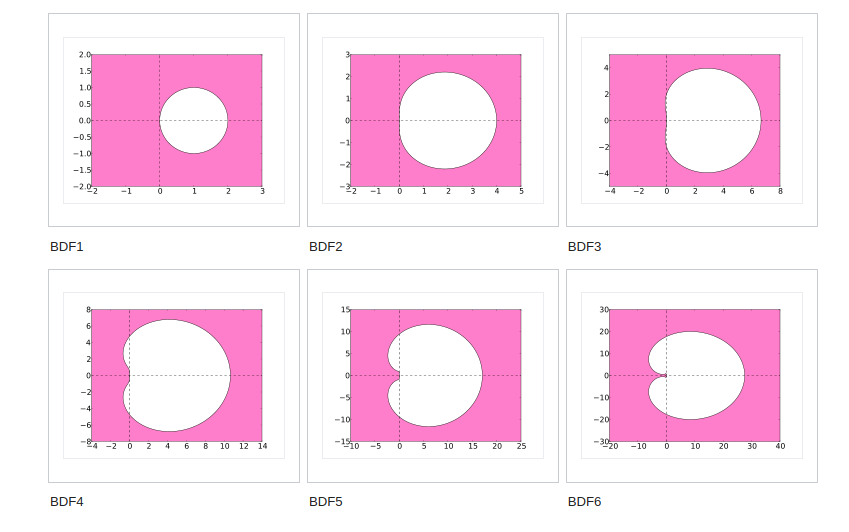
\includegraphics[height=3in]{fig/stabilityDomain.png}
  %\caption{fig1}
 
\end{figure}
\end{solution}

